\documentclass[11pt]{article}

\usepackage[english]{babel}


\usepackage{graphicx}
\usepackage[colorlinks=true, allcolors=blue]{hyperref}

\usepackage[title]{appendix}

\usepackage{amssymb,amsmath,amsthm,amsfonts,amstext}
\usepackage[left=1.5cm,right=1.5cm,top=1.5cm,bottom=1.5cm]{geometry}
\usepackage{enumerate}

\usepackage[mathscr]{euscript}

\usepackage{soul}

\newcommand{\redtext}[1]{{\color{red}{#1}}}
\newcommand{\bluetext}[1]{{\color{blue}{#1}}}
\newcommand{\greentext}[1]{{\color{green}{#1}}}
\newcommand{\browntext}[1]{{\color{brown}{#1}}}
\newcommand{\orangetext}[1]{{\color{orange}{#1}}}


\usepackage{tikz}
\usetikzlibrary{arrows}
\usetikzlibrary{arrows.meta}
\usetikzlibrary{shapes}
\usetikzlibrary{backgrounds}
\usetikzlibrary{positioning}
\usetikzlibrary{decorations.markings}
\usetikzlibrary{patterns}
\usetikzlibrary{calc}
\usetikzlibrary{fit}
\usetikzlibrary{decorations}
\usetikzlibrary{decorations.pathreplacing}

\usepackage[framemethod=TikZ]{mdframed}

\usepackage[noend]{algpseudocode}
\makeatletter
\def\BState{\State\hskip-\ALG@thistlm}
\makeatother

\usepackage[ruled]{algorithm2e}
\renewcommand{\algorithmcfname}{Algorithm}
\newtheorem{mdalgorithm}{Algorithm}
\newenvironment{Algorithm}{\begin{ourbox}\begin{mdalgorithm}}{\end{mdalgorithm}\end{ourbox}}
\newenvironment{ourbox}{\begin{mdframed}[hidealllines=false,innerleftmargin=10pt,backgroundcolor=white!10,innertopmargin=2pt,innerbottommargin=5pt,roundcorner=10pt]}{\end{mdframed}}


\newtheorem{theorem}{Theorem}
\newtheorem{corollary}[theorem]{Corollary}
\newtheorem{proposition}[theorem]{Proposition}
\newtheorem{lemma}[theorem]{Lemma}
\newtheorem{fact}{Fact}
\newtheorem{claim}[theorem]{Claim}
\newtheorem*{remark}{Remark}
\newtheorem{definition}{Definition}
\newtheorem{example}{Example}
\newtheorem{conjecture}{Conjecture}


\newenvironment{proofof}[1]{\begin{proof}\textcolor{red}{TOPROVE 0}\end{proof}}

\newcommand\IGNORE[1]{}

\newcommand\lpopt{\hbox{\text{LP}$_{\text{opt}}$}}
\newcommand\sm{\backslash}

\newcommand{\R}{\ensuremath{\mathbb R}}
\newcommand{\Rp}{\ensuremath{\R_{\geq 0}}}
\newcommand{\Q}{\ensuremath{\mathbb Q}}
\newcommand{\Qp}{\ensuremath{\Q_{\geq 0}}}
\newcommand{\Zint}{\ensuremath{\mathbb Z}}
\newcommand{\Zp}{\ensuremath{\Zint_{\geq 0}}}

\newcommand{\opt}{\textsc{opt}}
\newcommand{\safe}{\mathscr{S}}
\newcommand{\unsafe}{\mathscr{U}}

\newcommand{\fgc}{\mathrm{FGC}}
\newcommand{\pqfgc}{(p,q)\text{-}\fgc}
\newcommand{\ponefgc}{(p,1)\text{-}\fgc}
\newcommand{\ptwofgc}{(p,2)\text{-}\fgc}
\newcommand{\pthreefgc}{(p,3)\text{-}\fgc}
\newcommand{\oneonefgc}{(1,1)\text{-}\fgc}
\newcommand{\oneqfgc}{(1,q)\text{-}\fgc}
\newcommand{\oneqplusfgc}{(1,q+1)\text{-}\fgc}
\newcommand{\pfourfgc}{(p,4)\text{-}\fgc}
\newcommand{\twopfourfgc}{(2p,4)\text{-}\fgc}


\newcommand{\As}{\mathscr{A}} 
\newcommand{\C}{\mathscr{C}} 
\newcommand{\F}{\mathcal{F}} 
\newcommand{\Ls}{\mathscr{L}} 
\newcommand{\Ps}{\mathscr{P}} 
\newcommand{\Ss}{\mathscr{S}} 
\newcommand{\T}{\mathscr{T}} 
\newcommand{\J}{{J}}


\newcommand{\alg}{\textsc{alg}}

\newcommand{\twoqfgc}{(2,q)\text{-}\fgc}

\newcommand\capbound{\lambda}

\newcommand\hG{\hat{G}}
\newcommand\hE{\hat{E}}
\newcommand\hV{\hat{V}}
\newcommand\hu{\hat{u}}

\newcommand{\pliableapx}{5}

\newcommand{\oneqfgcapx}{7}

\newcommand\ASC{\mathrm{Cover\,Small\,Cuts}}
\newcommand\twoASC{\mathrm{2\text{-}Cover\,Small\,Cuts}}
\newcommand\threeASC{\mathrm{3\text{-}Cover\,Small\,Cuts}}

\newcommand{\alphatwo}{2}

\newcommand{\row}{\hbox{\textsl row}}


\title{Improved Approximation Algorithms for Flexible Graph Connectivity and Capacitated Network Design}

\author{\large
Ishan Bansal\thanks{
        {\tt ib332@cornell.edu}.
	Amazon, Bellevue, WA, USA. This work is external and does not relate to the position at Amazon. }
\and
Joseph Cheriyan\thanks{
{\tt jcheriyan@uwaterloo.ca}.
        Department of Combinatorics \& Optimization, University of Waterloo, Canada.}
\and
Sanjeev Khanna\thanks{
        {\tt sanjeev@cis.upenn.edu}.
        University of Pennsylvania, Philadelphia, PA, USA.}
\and 
Miles Simmons\thanks{
        {\tt mjsimmons@uwaterloo.ca}.
        Department of Combinatorics \& Optimization, University of Waterloo, Canada.}
}

\begin{document}
\maketitle


\begin{abstract}{
We present improved approximation algorithms for some problems in
the related areas of Flexible Graph Connectivity and Capacitated Network Design.
In the $(p,q)$-Flexible Graph Connectivity problem, denoted $\pqfgc$, 
the input is a graph $G(V, E)$ where $E$ is partitioned into {\em safe} and {\em unsafe} edges, and the goal is to find a minimum cost set of edges $F$ such that the subgraph $G'(V, F)$ remains $p$-edge connected upon removal of any $q$ unsafe edges from $F$. In the related Cap-$k$-ECSS problem, we are given a graph $G(V,E)$ whose edges have arbitrary integer capacities, and the goal is to find a minimum cost subset of edges $F$ such that the graph $G'(V,F)$ is $k$-edge connected.

We obtain a $\oneqfgcapx$-approximation algorithm for the $\oneqfgc$ problem that improves upon the previous best $(q+1)$-approximation. We also give an $O(\log{k})$-approximation algorithm for the Cap-$k$-ECSS problem, improving upon the previous best $O(\log{n})$-approximation whenever $k = o(n)$. Both these results are obtained by using natural LP relaxations strengthened with the knapsack-cover inequalities, and then during the rounding process utilizing an $O(1)$-approximation algorithm for the problem of covering small cuts. 
We also show that the the problem of covering small cuts inherently arises in another variant of $\pqfgc$. Specifically, we show $O(1)$-approximate reductions between the $\twoqfgc$ problem and the $\twoASC$ problem where each small cut needs to be covered twice.
}
\end{abstract}

\section{Introduction \label{sec:intro}}

We study some problems in the related areas of Flexible Graph Connectivity and Capacitated Network Design.

\subsection*{Flexible Graph Connectivity and the $(p,q)$-FGC problem}

Adjiashvili, Hommelsheim and M\"uhlenthaler \cite{AHM21}
introduced the model of Flexible Graph Connectivity that we denote by $\fgc$ as a way to model network design problems where edges have non-uniform reliability. 
Boyd, Cheriyan, Haddadan and Ibrahimpur \cite{BCHI23} introduced a
generalization of $\fgc$, called $(p,q)$-Flexible Graph Connectivity problem, denoted $\pqfgc$, where $p$ is
an integer denoting {\em connectivity} requirement, and $q$ is an integer denoting the {\em robustness} requirement.
An instance of $\pqfgc$ consists of an undirected graph $G = (V,E)$, where $E$ is partitioned into
a set of safe edges $\safe$ (edges that never fail) and a set of unsafe edges $\unsafe$ (edges that may fail),
and nonnegative edge-costs $c \in \Qp^E$.  A subset $F \subseteq
E$ of edges is feasible for the $\pqfgc$ problem if for any set
$F'$ consisting of at most $q$ unsafe edges, the subgraph $(V, F-F')$
remains $p$-edge connected. The objective is to find a
feasible solution $F$ that minimizes $c(F) = \sum_{e \in F} c_e$.

Boyd et al.\ \cite{BCHI23} presented a $4$-approximation algorithm
for $\ponefgc$ based on the
primal-dual method of Williamson, Goemans, Mihail \& Vazirani (WGMV) \cite{WGMV95}, and a
$(q+1)$-approximation algorithm for $\oneqfgc$; moreover, they gave
an $O(q \log n)$-approximation algorithm for (general) $\pqfgc$.
Subsequently, numerous results and approximation algorithms have been presented by
Bansal, Bansal et~al., Chekuri \& Jain, Nutov, etc., see \cite{B2023,BCGI24,CJ23,N2024}.


\subsection*{Capacitated Network Design and the Cap-$k$-ECSS problem}

The Cap-$k$-ECSS problem is as follows:
Given an undirected graph $G = (V,E)$ with edge costs $c \in \Qp^E$ and
edge capacities $u \in \mathbb{Z}_{\geq 0}^E$, find a minimum-cost
subset of the edges $F\subseteq E$ such that the capacity of any
cut in $(V,F)$ is at least $k$.
Let $u_{min}$ (respectively, $u_{max}$) denote the minimum (respectively,
maximum) capacity of an edge in $E$, and assume (w.l.o.g.) that $u_{max} \leq k$.

The best known approximation ratio for Cap-$k$-ECSS is
$\min(O(\log{|V|}), k, 2u_{max}, \pliableapx \cdot {\lceil k/u_{min} \rceil})$, due to
Chakrabarty et~al., Goemans et~al., \& Bansal \cite{CCKK15,GGPSTW94,B2023}.

For a graph $G=(V,E)$ and a set of nodes $S\subseteq{V}$, the \textit{cut of $S$}, denoted by $\delta(S)$, refers to the set of edges that have exactly one end-node in $S$. We call a cut $\delta(S)$ \textit{nontrivial} if $S$ is a nonempty, proper subset of $V$, that is, if $\emptyset\neq{S}\subsetneq{V}$. 

The following integer program formulates the Cap-$k$-ECSS problem.

\begin{align*}\label{intro-IP:CapkECSS}
    \min\;\;&\sum_{e\in E}c_e x_e \tag{IP: CapkECSS}\\
    \text{s.t.}\;\;& \sum_{e\in E\cap \delta(S)} u_ex_e \geq k && \forall\;\; \emptyset\subsetneq S\subsetneq V \\
    &x_e\in \{0,1\} && \forall\;\; e\in{E}
\end{align*}

The LP (linear programming) relaxation of the above integer program
is obtained by replacing $x_e\in\{0,1\}$ by $0\leq x_e\leq 1$,
$\forall e\in{E}$.
The following well-known example shows that the LP relaxation has
integrality ratio $\Omega(k)$.

The graph $G$ consists of a pair of nodes, and a pair of parallel
edges $e_1, e_2$ between the two nodes.  Edge $e_1$ has cost zero
and capacity $k-1$, and edge $e_2$ has cost~one and capacity $k$.
A feasible solution of the integer program has cost~one (since $e_2$ must be picked).
On the other hand, a feasible solution $x$ to the LP relaxation of cost $1/k$ is given
by $x_{e_1}=1, x_{e_2}=1/k$.


\subsection*{Knapsack-Cover Inequalities (KCI) for Capacitated Network Design}
{
The LP relaxation of \eqref{intro-IP:CapkECSS} can be strengthened
using the Knapsack-Cover Inequalities (KCI). For any non-trivial
cut $S$ and a subset of the edges $A\subseteq E$, the following is
a valid inequality for all integer solutions of \eqref{intro-IP:CapkECSS}.

\begin{align*}
        \sum_{e\in E\cap\delta(S) - A} u_e(A,S) x_e \geq D(A,S)
\end{align*}
where $D(A,S) = \max\{0,k - \sum_{e\in \delta(S)\cap A} u_e\}$ and
$u_e(A,S) = \min\{u_e,D(A,S)\}$.
(By plugging in $A=\emptyset$, we get the constraint
$\sum_{e\in E\cap\delta(S)} u_e x_e \geq k$,
which is a constraint of \eqref{intro-IP:CapkECSS}.)

We add these inequalities to \eqref{intro-IP:CapkECSS} to obtain the
following LP relaxation of the Cap-$k$-ECSS problem.

\begin{align*}\label{intro-KCLP:CapkECSS}
    \min\;\;&\sum_{e\in E}c_e x_e \tag{KCLP:~CapkECSS}\\
    \text{s.t.}\;\;& \sum_{e\in E\cap\delta(S) - A} u_e(A,S) x_e \geq D(A,S) && \forall\;\; \emptyset\subsetneq S\subsetneq V, A\subseteq E \\
    &0 \leq x_e \leq 1 && \forall\;\; e\in E
\end{align*}

Observe that this LP has a number of constraints that is exponential
in the size of the input~instance (of Cap-$k$-ECSS).
By following the cut-and-round approach employed by
Carr, Fleischer, Leung \& Phillips \cite{CFLP00},
one can round this LP in polynomial time
to an approximately optimal integer solution
via the ellipsoid~method by designing an efficient pseudo-separation subroutine.
See sections~\ref{sec:oneqfgc}, \ref{sec:twoqfgc}, \ref{sec:logk-approx} for details.
}

\subsection*{LP relaxations for $(p,q)$-FGC}
{
The following linear program gives a lower bound on the optimal solution value for $(p,q)$-FGC.
Such LP relaxations are discussed in \cite{BCHI23} and \cite[Section~2]{CJ23}.

To motivate the LP relaxation, consider an auxiliary capacitated graph
that has the same set of nodes and the same set of edges as the
graph of the $(p,q)$-FGC instance.
Assign a capacity of $(p+q)$ to each safe edge and a capacity of $p$ to each unsafe edge.
Let $k=p(p+q)$ and view the capacitated graph as an instance of the Cap-$k$-ECSS problem.
In general, observe that a feasible solution of the $(p,q)$-FGC instance corresponds
to a feasible solution of the Cap-$k$-ECSS instance, but not vice-versa.
(When either $p=1$ or $q=1$, then a feasible solution of the Cap-$k$-ECSS instance
corresponds to a feasible solution of the $(p,q)$-FGC instance.)
Our LP relaxation can be viewed as the natural ``cut covering'' LP relaxation
of the Cap-$k$-ECSS problem.
Each safe edge $e$ has a variable $x_e$, each unsafe edge $f$ has a variable $y_f$,
and for any set of nodes $S$, we use the notation
$x(\delta(S)) \equiv \sum\{x_e \mid e\in\delta(S)\cap\safe\}$,
$y(\delta(S)) \equiv \sum\{y_f \mid f\in\delta(S)\cap\unsafe\}$.

\begin{align}
	\lpopt := \quad \min  & \sum_{e \in \safe} c_e x_e + \sum_{f \in \unsafe} c_f y_f & \label{eq:obj} \\
	\text{s.t.} \quad & (p) y(\delta(S)) + (p+q) x(\delta(S)) \geq p(p+q)  & \forall \quad \emptyset \subsetneq S \subsetneq V \label{eq:twoec} \\
& 0 \leq x_e \leq 1 & \forall e\in\safe	\label{eq:nonneg} \\
& 0 \leq y_f \leq 1 & \forall f\in\unsafe
\end{align}
}

\subsection*{The $f$-connectivity problem and Jain's iterative rounding algorithm}
{
Most connectivity augmentation problems can be formulated in
a general framework called $f$-connectivity. In this problem, we
are given an undirected graph $G = (V,E)$ on $n$ nodes with
nonnegative costs $c \in \Qp^E$ on the edges and a requirement
function $f:2^V\to\Zp$ on subsets of nodes.
We are interested in finding an edge-set $\J \subseteq E$ with minimum
cost $c(\J) := \sum_{e \in \J} c_e$ such that for all cuts
$\delta(S),\ S \subseteq V$, we have
$|\delta(S) \cap \J| \geq f(S)$.
This problem can be formulated as the following integer program
where the binary variable $x_e$ models the inclusion of the edge $e$ in $\J$:
\begin{align*} \tag{IP: $f$-connectivity}
\label{eq:fconnectivityIP}
\min \quad \qquad		& \quad \sum_{e \in E} c_e x_e 		& \\
\text{subject to: } 	& \quad x( \delta(S) ) \geq f(S) 	& \forall \, \, S \subseteq V \\
					& \quad x_e \in \{0,1\} & \forall \, \, e \in E. \\
\end{align*}
Assuming that the function $f$ is weakly supermodular, \st{(and integral)} {integral, and has a positive value for some $S\subset{V}$},
Jain \cite{Jain01} presented a 2-approximation algorithm for the $f$-connectivity problem.
Recently, Dinitz et al.\ \cite{DKK22,DKKN23} discussed extensions of Jain's methods to
the setting of locally weakly supermodular functions and weakly
{$\F$}-supermodular functions.  In section~\ref{sec:twoqfgc}, we
use the latter notion. 


Let $\F$ be a family of subsets of $V$, such that $\emptyset,V \notin \F$.
A function $f$ is called \textit{weakly $\F$-supermodular} if,
{ $f(S)=0,\,\forall{S\not\in\F}$, and } for
all $A,B \in \F$, at least one of the following holds:
\begin{itemize}
    \item $A - B, B - A \in \F$ and $f(A) + f(B) \leq f(A - B) + f(B - A)$
    \item $A \cap B, A \cup B \in \F$ and $f(A) + f(B) \leq f(A \cap B) + f(A \cup B)$
\end{itemize}


\begin{remark}
The reader can follow our presentation independently of \cite{DKKN23}; nevertheless, we mention that \cite{DKKN23} has a few typos, and there is confusion pertaining to the functions $f$ and $f_{\F}$. Our presentation does not use the notion of $f_{\F}$ and our definition of a weakly $\F$-supermodular function $f$ adds the condition $f(S)=0,\,\forall{S\not\in\F}$.
\end{remark}


The following result is an extension of \cite[Theorem~2.5]{Jain01}.

\begin{proposition}
Let $G$ be a graph and let $x\in\{0,1\}^{E(G)}$ denote a subgraph of $G$.
Let $f: 2^{V(G)} \rightarrow \Zint$ be a weakly $\F$-supermodular function.
Then $f(S) - |\delta_x(S)|$ is also a weakly $\F$-supermodular function.
\end{proposition}

Moreover, \cite[Lemma~4.1]{Jain01} holds when the function $f$
is a weakly $\F$-supermodular function.
Let us call a node~set $S$ \textit{tight} if $x(\delta(S)) = f(S)$,
and let $\chi^S$ denote the incidence vector of $\delta(S)$.
\cite[Lemma~4.1]{Jain01} states that if $A,B \subseteq V(G)$ are tight sets,
then either $A-B, B-A$ are tight sets and
$\chi^A + \chi^B = \chi^{A-B} + \chi^{B-A}$, or 
$A\cap{B}, A\cup{B}$ are tight sets and
$\chi^A + \chi^B = \chi^{A\cap{B}} + \chi^{A\cup{B}}$.

The other relevant lemmas and theorems of \cite{Jain01} continue
to hold for a weakly $\F$-supermodular function $f$; in particular,
\cite[Theorem~3.1]{Jain01} holds; it states that for any basic
solution $x$ of the LP relaxation of the $f$-connectivity problem,
there is an edge $e$ such that $x_e\geq{1/2}$.


In section~\ref{sec:twoqfgc}, we define requirement functions $f$ of the form
\[
f(S) = \begin{cases}
    k, &\text{ if } \emptyset\neq{S}\subsetneq{V} \text{ and } |\delta(S)\cap E_0| \leq 1 \\ 0, &\text{ otherwise},
\end{cases}
\]
where $k$ is a positive integer and $E_0$ is a subset of $E(G)$.
Let $\F$ be the family of nonempty, proper subsets $S$ of $V(G)$
such that $|\delta(S)\cap{E_0}| \leq1$.
For any two sets $A,B\in\F$, either $A-B,B-A\in\F$ or $A\cap{B},A\cup{B}\in\F$;
this can be proved via case analysis;
for example, see the last part of the proof of \cite[Lemma~4.3]{BCHI23}.
Hence, it follows that the above requirement function $f$ is weakly $\F$-supermodular.
This gives the next result.

\begin{proposition} \label{prop:wFsupmod}
Jain's iterative rounding algorithm finds a 2-approximate solution
to an $f$-connectivity problem and a pre-selected edge~set $E_0$
such that $f$ has the form
$\displaystyle f(S) = \begin{cases}
    k, &\text{ if } \emptyset\neq{S}\subsetneq{V} \text{ and } |\delta(S)\cap E_0| \leq 1 \\ 0, &\text{ otherwise}.
\end{cases}
$
\end{proposition}
}

\subsection*{The $\ASC$ problem}
We follow the notation from \cite[Section~1.3]{BCGI:arxiv}.
In an instance of the $\ASC$ problem, we are given an
undirected capacitated graph $G = (V,E)$ with edge-capacities $u
\in \Qp^E$, a set of links $L \subseteq \binom{V}{2}$ with costs
$c \in \Qp^L$, and a threshold $\capbound \in \Qp$.
A subset $F \subseteq L$ of links is said to \emph{cover} a
node-set $S$ if there exists a link $e \in F$ with exactly one
end-node in $S$.
The objective is to find a minimum-cost $F\subseteq{L}$ that covers
each non-empty $S \subsetneq V$ with $u(\delta_E(S)) < \capbound$.

Let $\C = \{ \emptyset \neq S \subsetneq V : u(\delta_E(S)) < \capbound \}$.
Then we have the following covering~LP relaxation of the problem.
\begin{align*}\label{LP:ASC} \tag{LP:\,{Cover\,Small\,Cuts}}
\min \quad \qquad		& \quad \sum_{f \in L} c_f x_f 		& \\
\text{subject to: } 	& \quad \sum_{f\in L\cap\delta(S)} x_f \geq 1 	& \forall \, \, S \in \C \\
					& \quad 0\leq x_f \leq 1 & \forall \, \, f \in L. \\
\end{align*}

The first constant-factor approximation algorithm was presented by
Bansal et~al., \cite{BCGI24}, and the approximation ratio was
improved from~16 to~10 by Nutov, \cite{N2024}, then from~10 to~5
by Bansal, \cite{B2023}.
The following result is due to Bansal, \cite{B2023}.

\begin{proposition} \label{prop:approxASC}
Given an instance of $\ASC$, the WGMV primal-dual algorithm, \cite{WGMV95}, finds
a feasible solution of cost $\leq \pliableapx\,\lpopt$ in polynomial time,
where $\lpopt$ denotes the optimal value of \eqref{LP:ASC}.
\end{proposition}

In section~\ref{sec:twoqfgc}, we also discuss the $\twoASC$ problem.
The inputs are the same as above, namely, $G=(V,E), u, L, c, \capbound$.
A subset $F \subseteq L$ of links is said to \emph{two-cover} a
node-set $S$ if $|F\cap\delta(S)|\geq2$, that is,
if there exist a pair of (distinct) links $e,e' \in F$
such that each of $e$ and $e'$ has exactly one end-node in $S$.
The objective is to find a minimum-cost $F\subseteq{L}$ that two-covers
each non-empty $S \subsetneq V$ with $u(\delta_E(S)) < \capbound$.

\subsection*{Our results}

We present improved approximation algorithms for the $\pqfgc$ problem and the Cap-$k$-ECSS problem.
In particular, we present the following results.
\begin{itemize}
\item A $\oneqfgcapx$-approximation algorithm for the $\oneqfgc$ problem.

\item $O(1)$-approximate reductions between the $\twoqfgc$ problem and the $\twoASC$ problem.

\item An $O(\log{k})$ approximation algorithm for the Cap-$k$-ECSS problem.

\item Moreover, we present two auxiliary results in the appendices.
The first one is motivated by the question:
For what values of the parameters $p$ and $q$ can one formulate
the $\pqfgc$ problem as an equivalent Cap-$k$-ECSS problem?
We show that one can formulate a $\pqfgc$ problem as an equivalent
Cap-$k$-ECSS problem if and only if $p=1$ or $q=1$.
Our second auxiliary result gives a (randomized) $O(p\log{n})$
approximation algorithm for the $\pqfgc$ problem, based on a result of Chekuri \& Quanrud \cite{CQ:soda19}.
\end{itemize}


\section{A $\oneqfgcapx$-Approximation Algorithm for $\oneqfgc$ \label{sec:oneqfgc}}
{
This section presents a $\oneqfgcapx$-approximation algorithm for the $(1,q)$-FGC problem.
For the convenience of the reader, the presentation in this section is independent of the rest of the paper. 

Our starting point is the natural LP relaxation that follows from taking a capacitated network design view of the problem whereby we assign each unsafe edge $e \in \unsafe$ has capacity $u_e=1$, and
each safe edge $e \in \safe$ has capacity $u_e=(q+1)$. The natural LP relaxation then seeks to minimize the total cost of edges subject to the constraint that $\forall\;\; \emptyset\subsetneq S\subsetneq V$, we have $\sum_{e\in\safe\cap\delta(S)} (q+1) x_e + \sum_{e\in\unsafe\cap\delta(S)} x_e \geq (q+1).$

It is easy to see that any $0/1$-valued solution to this LP is a valid solution to a given instance of  $\oneqfgc$, and vice versa.
However, it is also easy to show that this LP has an integrality gap of $q$ by adapting the integrality gap example we saw earlier for the Cap-$k$-ECSS problem. We consider an instance consisting of a pair of nodes connected by $q$ parallel unsafe edges of cost $0$, and a single safe edge of cost $1$. Now the optimal fractional solution has cost $1/q$ while the optimal integral solution has cost $1$.


To get around this integrality gap, we strengthen the LP relaxation of $\oneqfgc$ using the knapsack-cover inequalities to obtain the following stronger LP. Intuitively, the added knapsack-cover constraint ensures that if a safe edge is being used to cover a cut that is partly being covered by unsafe edges, say by $k$ of them, then the capacity of the safe edge is reduced to $(q+1)-k$.

\begin{align*}\label{KCLP:oneqfgc}
    \min\;\;&\sum_{e\in E}c_e x_e \tag{KCLP:$(1,q)$-FGC}\\
    \text{s.t.}\;\;& \sum_{e\in\safe\cap\delta(S)} (q+1) x_e + \sum_{e\in\unsafe\cap\delta(S)} x_e \geq (q+1) && \forall\;\; \emptyset\subsetneq S\subsetneq V \\
    & \sum_{e\in E\cap\delta(S) - A} u_e(A,S) x_e \geq D(A,S) && \forall\;\; \emptyset\subsetneq S\subsetneq V, A\subseteq E \\
    &0 \leq x_e \leq 1 && \forall\;\; e\in E,
\end{align*}

where $D(A,S) = \max\{0,\, (q+1)-\sum\{ u_e \mid e\in{A}\cap\delta(S)\}\}$, and $u_e(A,S) = \min\{u_e,\, D(A,S)\}$.
We would like to solve the above LP using the ellipsoid method, but, unfortunately, we do not know a polynomial-time separation oracle for knapsack-cover inequalities. We will instead identify a subset of unsafe edges $A$, and a polynomial-time computable collection of cuts such that as long as the knapsack-cover inequalities hold for this collection, we will be able to show that the integrality gap of the fractional solution is at most $\oneqfgcapx$. We can use this property to design a polynomial-time algorithm. In what follows, we assume w.l.o.g.\ that the optimal LP solution cost, say $\lpopt$, is known as it can be identified via binary search. We can thus replace the minimization objective with a feasibility constraint on our solution, namely, $\sum_{e\in E}c_e x_e \leq \lpopt$.



\begin{lemma}\label{lem:polytimeKC-oneqfgc}
There is a polynomial-time algorithm that computes a solution $x^*$ to \eqref{KCLP:oneqfgc} of value at most $\lpopt$ such that the solution satisfies the following two properties:

\begin{itemize}
\item[(P1)]
$\sum_{e\in\safe\cap\delta(S)} (q+1) x^*_e + \sum_{e\in\unsafe\cap\delta(S)} x^*_e \geq (q+1)$.

\item[(P2)]
Let $A = \{ e \in  \unsafe~|~x^*_e \ge 2/7 \}.$
For any nonempty ${S}\subsetneq{V}$,
if $\sum_{e\in\safe\cap\delta(S)} (q+1) x^*_e +
\sum_{e\in\unsafe\cap\delta(S)} x^*_e \leq 2(q+1)$, then
$$\sum_{e\in E\cap\delta(S) - A} u_e(A,S) x_e \geq D(A,S).$$
\end{itemize}
\end{lemma}
\begin{proof}\textcolor{red}{TOPROVE 1}\end{proof}



\noindent
{\bf The Rounding Algorithm:}
Given a solution $x^*$ of cost at most $\lpopt$ that satisfies (P1) and (P2), Algorithm~\ref{alg:oneq-FGC}, presented below, rounds it to an integral solution of cost at most $7\lpopt$. We describe here the main idea of our rounding scheme. 

We say a non-trivial cut $\delta(S)$ is a {\em small cut} if $\sum_{e\in \unsafe_1\cap\delta(S)}u_e \;+\; \sum_{e\in \unsafe_2\cap\delta(S)}\frac{7}{2} u_ex^*_e < (q+1)$ where $\unsafe_{1} = \{e\in \unsafe : x^*_e \geq 2/7\}$, and $\unsafe_{2} = \unsafe \setminus \unsafe_1$.
To handle the presence of small cuts, we will first show that the solution $x^*$ restricted to safe edges and scaled up by a factor of $7/5$ constitutes a feasible solution to the $\ASC$ instance defined by small cuts (see Lemma~\ref{lem:oneqfgc1}). We can thus pick a set $\safe_1$ of safe edges by applying the 5-approximation algorithm of \cite{B2023,BCGI24} to this instance of the $\ASC$ problem, getting a solution whose cost is at most $7$ {times} as large as the cost of $x^*$ restricted to safe edges. After this step, we can contract connected components formed by edges in $\safe_1$, and get a new instance that does not have any small cuts. 
Since there are no small cuts, we can get a feasible solution for the $f$-connectivity problem where $f(S) = q+1$ for every non-trivial cut $\delta(S)$ by 
taking all edges in $\unsafe_1$ and scaling up $x^*$ restricted to $\unsafe_2$ by a factor of $7/2$.
Since $f$ is weakly supermodular, we can apply Jain's iterative rounding scheme~\cite{Jain01} to solve this $f$-connectivity problem and recover a $2$-approximate solution, giving us an integral solution whose cost is at most $7$ {times} as large as the cost of $x^*$ restricted to unsafe edges (see Lemma~\ref{lem:oneqfgc2}).
Thus, we get an integral solution whose total cost of safe and unsafe edges is bounded by at most $7$ times the LP cost.

{
 \begin{algorithm}
     \caption{$\oneqfgcapx$-approximate solution to $(1,{q})$-FGC} \label{alg:oneq-FGC}
     \begin{algorithmic}[1]
         \Require Graph $G=(V,E)$ where $E$ is partitioned into $\safe\bigcup\unsafe$, with edge costs $\{c_e\}_{e\in E}$.  A solution $x^*$ to \eqref{KCLP:oneqfgc} as promised by Lemma~\ref{lem:polytimeKC-oneqfgc}.
         \State $\unsafe_{1} \gets \{e\in \unsafe : x^*_e \geq 2/7\}$, and $\unsafe_{2} \gets \unsafe - \unsafe_1$.
         \State
		\vspace{-4ex}
		{\begin{itemize}
             \item[(a)] Apply the approximation~algorithm for $\ASC$ on the instance with
		$G'=(V,E' = \unsafe)$,
		where each edge of $\unsafe_1$ is given unit capacity,
		each edge $e\in\unsafe_2$ is given capacity ${7/2}\,x^*_e$,
		and with link set $\safe$.
		Define the threshold $\lambda$ (for Small~Cuts) to be $(q+1)$. Thus, we have:
\[
\sum_{e\in \unsafe_1\cap\delta(S)}u_e \;+\; \sum_{e\in \unsafe_2\cap\delta(S)}\frac{7}{2} u_ex^*_e < (q+1) \tag{definition of {\em small cuts}}
\]
             \item[(b)]  Let the output of the call in step~(a) be denoted $\safe_{1}$.
		\end{itemize}}
         \State Construct a graph $G''=(V,\unsafe_{2})$ where each edge $e\in \unsafe_{2}$ has cost $c_e$.
		Define the requirement of a non-trivial cut $\delta(S)$ to be
$$f(S) = \max\{ 0,\;\; (q+1) - ((q+1) |\delta(S)\cap \safe_{1}| + |\delta(S)\cap \unsafe_{1}|) \}.$$
		This function $f$ is weakly supermodular, so a 2-approximate solution for
		this instance of $f$-connectivity can be computed using Jain's
		iterative rounding method \cite{Jain01}.
         \State Return the union of the set of unsafe~edges picked by the previous step (via the iterative rounding algorithm) and $\safe_{1} \cup \unsafe_{1}$.
     \end{algorithmic}
 \end{algorithm}
}


The next two lemmas formalize the key properties of the solution $x^*$ that are used in the rounding scheme above, allowing us to show that it indeed returns a feasible integral solution of cost at most 
$\oneqfgcapx\ c(x^*)$.

{
\begin{lemma}\label{lem:oneqfgc1}
In step~2 of Algorithm~\ref{alg:oneq-FGC}, a feasible fractional
solution to the CoverSmallCuts instance is given by
	$\hat{x}_e = \min\{1,\, \frac{7}{5} x^*_e\}$ for $e\in \safe$.
\end{lemma}

\begin{proof}\textcolor{red}{TOPROVE 2}\end{proof}

\begin{lemma}\label{lem:oneqfgc2}
In step~3 of Algorithm~\ref{alg:oneq-FGC}, a feasible fractional
solution to the $f$-connectivity problem is given by
	$x'_e = \frac{7}{2} x^*_e$ for $e\in \unsafe_{2}$.
\end{lemma}

\begin{proof}\textcolor{red}{TOPROVE 3}\end{proof}

The output of Algorithm~\ref{alg:oneq-FGC} is feasible for the
$\oneqfgc$ problem due to the definition of the $f$-connectivity
problem in step~3 of the algorithm. The cost of the edges in
$\unsafe_{1}$ is $\leq {7/2} \sum_{e\in \unsafe_{1}}x^*_e c_e$ since
$x^*_e \geq 2/7$ for each edge $e$ in $\unsafe_{1}$. Additionally,
the cost of the edges in $\safe_1$ is $\leq 7 \sum_{e\in \safe_1}x^*_e c_e$
by Lemma~\ref{lem:oneqfgc1} and by Proposition~\ref{prop:approxASC}.
Lastly, the cost of the edges returned by Jain's iterative rounding
algorithm in step~3 of Algorithm~\ref{alg:oneq-FGC} is at most
$\sum_{e\in \unsafe_{2}}(2)(7/2) c_e x^*_e = 7\,\sum_{e\in \unsafe_{2}}c_e x^*_e$,
by Lemma~\ref{lem:oneqfgc2}.
Putting it all together, the cost of the solution returned by
Algorithm~\ref{alg:oneq-FGC} is at most $\oneqfgcapx\ c(x^*)$.
}


\begin{theorem} \label{thm:approx-oneqfgc}
Let $\opt$ be the optimal solution value for a given instance of $\oneqfgc$. Then there is a polynomial-time algorithm that computes a solution $x^*$ to \eqref{KCLP:oneqfgc} of value at most $\opt$ (possibly satisfying only a subset of the constraints) and rounds it to obtain a feasible integer solution of cost at most $\oneqfgcapx\, \opt$.
\end{theorem}
}


\section{$O(1)$-Approximate Reductions between $\twoqfgc$ and $\twoASC$ \label{sec:twoqfgc}}
{
We provide reductions between the two problems $\twoqfgc$ and
$\twoASC$ in both directions.
Each of these reductions preserves the approximation ratio up to a constant factor.

Recall that in the $\twoASC$ problem,
we are given a graph $\hG=(\hV,\hE)$ with edge capacities $u$, a number $\capbound$,
as well as a set of links $L \subseteq \binom{\hV}{2}$ with link costs $c$;
the goal is to find a cheapest set of links $\J\subseteq{L}$
that two-covers the family of small cuts,
namely, $\{S\subsetneq{\hV}, S\not=\emptyset \mid u(\delta(S)) < \capbound\}$.

\subsection*{Reducing $\twoqfgc$ to $\twoASC$ with approximation ratio $O(1)$}
{
Suppose we have an LP~relative $\alpha$-approximation algorithm for $\twoASC$.
{
(In other words, suppose we have access to a polynomial-time algorithm that rounds
a given fractional feasible solution of the LP relaxation of $\twoASC$
to a feasible (integral) solution of cost $\leq \alpha\,\lpopt$, 
where $\lpopt$ denotes the optimal value of the LP~relaxation.)
}


Let $G=(V,E = \safe \cup \unsafe)$ be an instance of $\twoqfgc$
with edge costs  $c \in \Qp^E$.  We use the following linear
programming relaxation. Informally speaking,
the first type of constraints (see~(1) below) correspond to
a $\oneqplusfgc$ problem,
and the second type of constraints (see~(2) below) say that for each safe edge $f$,
the edges in $E-f$ should satisfy the requirements of $\oneqfgc$
(i.e., each nontrivial cut has one safe edge or $q+1$ edges).

\begin{align*}\label{LP:twoqfgc}
    \min\;\;&\sum_{e\in E}c_e x_e \tag{LP:$(2,q)$-FGC}\\
    \text{s.t.}\;\;& \sum_{e\in \safe \cap \delta(S)} (q+2)x_e + \sum_{e\in \unsafe \cap\delta(S)}x_e \geq q+2 && \forall\;\; \emptyset\subsetneq S\subsetneq V\tag{1} \\
    & \sum_{e\in (\safe - f)\cap \delta(S)} (q+1)x_e + \sum_{e\in \unsafe \cap\delta(S)}x_e \geq q+1 && \forall\;\; \emptyset\subsetneq S\subsetneq V,\;\;\forall\;\; f\in\safe \tag{2}\\
    &0\leq x\leq 1
\end{align*}

Each of the inequalities~(1) and each of the inequalities~(2) (for
each $f\in\safe$, $\forall S\subsetneq{V},S\not=\emptyset$) can be
strengthened using the knapsack-cover inequalities.  

{
We follow the method of section~\ref{sec:oneqfgc} for rounding this strengthened LP.
(Recall that no polynomial-time separation algorithm is known for
these knapsack-cover inequalities, hence, we have to work around this gap.)
We assume w.l.o.g.\ that $\lpopt$, the optimal value of the
strengthened LP, is known, since it can be identified via binary
search. Thus, we replace the minimization objective with a feasibility
constraint, namely, $\sum_{e\in E}c_e x_e \leq \lpopt$.
As in section~\ref{sec:oneqfgc}, we will design a polynomial-time
algorithm for rounding the strengthened LP by picking some sets of
unsafe edges, and a polynomial-time computable collection of cuts 
$\C$.  We will show that our rounding algorithm succeeds as long 
as the knapsack-cover inequalities hold for each set $S\in\C$ and
an appropriate set of unsafe edges $A$. 
}


{
\begin{lemma}\label{lem:polytimeKC-twoqfgc}
There is a polynomial-time algorithm that computes a solution $x^*$
to \eqref{LP:twoqfgc}
such that $\sum_e c_ex^*_e\leq\lpopt$ and, moreover, $x^*$ satisfies
the following properties:

\begin{itemize}
\item[(P3)]
$\sum_{e\in\safe\cap\delta(S)} (q+2) x^*_e +
\sum_{e\in\unsafe\cap\delta(S)} x^*_e \geq (q+2) \qquad\forall\;
        \emptyset\neq{S}\subsetneq{V}$.

\item[(P4)]
Let $A^{(1)} = \{ e \in  \unsafe~|~x^*_e \ge 2/7 \}.$
For any nonempty ${S}\subsetneq{V}$,
if $\sum_{e\in\safe\cap\delta(S)} (q+2) x^*_e +
\sum_{e\in\unsafe\cap\delta(S)} x^*_e \leq 2(q+2)$, then
$$\sum_{e\in E\cap\delta(S) - A^{(1)}} u_e(A^{(1)},S) x_e \geq D(A^{(1)},S).$$

\item[(P5)]
For each safe edge $f$,
$\sum_{e\in(\safe-f)\cap\delta(S)} (q+1) x^*_e +
\sum_{e\in\unsafe\cap\delta(S)} x^*_e \geq (q+1) \qquad\forall\;
        \emptyset\neq{S}\subsetneq{V}$.

\item[(P6)]
Let $A^{(2)} = \{ e \in  \unsafe~|~x^*_e \ge 1/2 \}.$
For each safe edge $f$ and for any nonempty ${S}\subsetneq{V}$,
if $\sum_{e\in(\safe-f)\cap\delta(S)} (q+1) x^*_e +
\sum_{e\in\unsafe\cap\delta(S)} x^*_e \leq 2(q+1)$, then
$$\sum_{e\in E\cap\delta(S) - A^{(2)}} u_e(A^{(2)},S) x_e \geq D(A^{(2)},S).$$
\end{itemize}
\end{lemma}

\begin{proof}\textcolor{red}{TOPROVE 4}\end{proof}
}


Our algorithm for rounding $x^*$ has two parts.
The first part applies the algorithm of section~\ref{sec:oneqfgc}
and finds a set of edges $\safe_0\cup\unsafe_0$ that is feasible
for the $\oneqplusfgc$ instance.
The second part uses the (assumed) $\alpha$-approximation algorithm
for $\twoASC$, as well as Jain's iterative rounding method, and finds
a set of edges $\safe_1\cup\safe_{\alg}\cup{\J}$.
Below, we show that the union of the two sets of edges is feasible
for $\twoqfgc$ and it has cost $\leq(4 \alpha + 11)\,c(x^*)$.

Next, we present the details of our algorithm and its analysis.

The first part simply applies the algorithm of section~\ref{sec:oneqfgc}
to round $x^*$ to an edge~set $\safe_0\cup\unsafe_0$ of cost
$\leq7\,c(x^*)$ that is feasible for the $\oneqplusfgc$ problem
(described by the inequalities~(1)), where $\safe_0$ is a set of
safe edges and $\unsafe_0$ is a set of unsafe edges.
(We mention that the fact that $x^*$ satisfies the inequalities~(2)
is not relevant for this part.)


In the second part of the algorithm, we start by
defining $\safe_1 = \{e\in\safe: x^*_e\geq 1/4\}$ and
$\unsafe_1 = \{e\in\unsafe: x^*_e\geq 1/2\}$.
Let $\safe_2 = \safe - \safe_1$ and
let $\unsafe_2 = \unsafe - \unsafe_1$.

Define $\C$ to be the family of all nontrivial cuts $\delta(S)$ such that
$|\unsafe_1\cap \delta(S)| + \sum_{e\in \unsafe_2 \cap\delta(S)} 2x^*_e < (q+1)$.


{
The analysis of the second part of our algorithm hinges on the next
lemma.  It shows that a (small) constant multiple of the fractional
vector $x^*_{\safe}$ is feasible for the LP~relaxation of the
$\twoASC$ instance defined by $\C$.

\begin{lemma} \label{lem:safepart-twoqfgc}
Let $x^*$ satisfy properties (P3)--(P6) of Lemma~\ref{lem:polytimeKC-twoqfgc}.
A feasible fractional solution to the $\twoASC$ instance defined
by $\C$ is given by the vector $(1_{\safe_1}, 4 x^*_{\safe_2})$; that is,
for any $\delta(S)\in\C$, we have
$|\safe_1\cap\delta(S)| \:+\: \sum_{e\in \safe_2\cap\delta(S)} 4x^*_e \:\:\geq\:\: 2$.
\end{lemma}

\begin{proof}\textcolor{red}{TOPROVE 5}\end{proof}
}


By Lemma~\ref{lem:safepart-twoqfgc}, we can use the $\alpha$-approximation
algorithm for $\twoASC$ to find a set of safe edges, call this set
$\safe_{\alg}$, that two-covers all the cuts in $\C$, incurring a
cost of $\leq4\alpha\, c(x^*_{\safe})$.


Now, for every nontrivial cut $\delta(S)$,
we either have $|\delta(S)\cap\safe_{\alg}|\geq2$, or we have
$|\delta(S)\cap\unsafe_1| + \sum_{e\in \unsafe_2 \cap\delta(S)} 2x^*_e \geq (q+1)$.

Next, we formulate an $f$-connectivity problem such that
a feasible solution to this problem will cover the nontrivial
cuts $\delta(S)$ with $|\delta(S)\cap\safe_{\alg}|<2$.

For a nontrivial cut $\delta(S)$ define,
\[
f(S) = \begin{cases}
    q+1, &\text{ if } \emptyset\neq{S}\subsetneq{V} \text{ and } |\delta(S)\cap \safe_{\alg}| \leq 1 \\
	0, &\text{otherwise}.
\end{cases}
\]

Observe that $(1_{\unsafe_1}, 2x^*_{\unsafe_2})$ is a fractional
feasible solution to the $f$-connectivity problem.
By Proposition~\ref{prop:wFsupmod}, Jain's iterative rounding
algorithm finds a feasible solution $\J\subseteq{\unsafe}$
to this $f$-connectivity problem of cost $\leq 4c(x^*_{\unsafe})$.


Finally, we claim that the union of the edge~sets found by the two
parts of the algorithm, namely, $E_{\alg}=(\safe_0\cup\unsafe_0)
\bigcup (\safe_1\cup\safe_{\alg}\cup\unsafe_1\cup{\J})$ is a feasible
solution of the $\twoqfgc$ instance, that is, every nontrivial cut
either has two safe edges (of $E_{\alg}$) or has $q+2$ edges (of $E_{\alg}$).
Consider any nontrivial cut $\delta(S)$ with at most one safe edge (of $E_{\alg}$).
If $\delta(S)\cap{E_{\alg}}$ has one safe edge, then $|\delta(S)\cap{\J}|\geq{q+1}$
(since $\J$ is feasible for the $f$-connectivity problem).
If $\delta(S)\cap{E_{\alg}}$ has no safe edges, then $|\delta(S)\cap{\unsafe_0}|\geq{q+2}$
(since $\safe_0\cup\unsafe_0$ is feasible for the $\oneqplusfgc$ problem).

Clearly, the cost of $E_{\alg}$ is $\leq 7\, c(x^*) + 4\alpha\,
c(x^*_{\safe}) + 4\, c(x^*_{\unsafe}) \leq (4\alpha+11)\, c(x^*)$.


{
\begin{theorem} \label{thm:approx-twoqfgc}
Suppose a polynomial-time LP~relative $\alpha$-approximation algorithm
for $\twoASC$ is available.

Then the above algorithm for $\twoqfgc$ runs in polynomial time and
returns a feasible (integral) solution of cost $\leq (4\alpha+11)\, \opt$,
where $\opt$ denotes the optimal value of the $\twoqfgc$ instance.
\end{theorem}
}

}


\medskip

\subsection*{Reducing $\twoASC$ to $\twoqfgc$ with approximation ratio $O(1)$}
{
In this subsection, we show that a $\beta$-approximation algorithm
for $(2,q)$-FGC implies an $(\beta+2)$-approximation algorithm for
unit-capacity $\twoASC$. 

Let $\hG=(\hV,\hE)$, $u$, $L$, $c$, $\capbound$ be an instance of
the unit-capacity $\twoASC$ problem; thus, each edge $e\in\hE$ has $u_e=1$.
The goal is to find a cheapest set of links that two-covers all the
nontrivial cuts $\delta(S)$ such that $|\delta(S)\cap\hE| <\capbound$.
Let $L^*$ denote an optimal solution, and let $\opt=c(L^*)$ denote its cost.


We map the above instance of $\twoASC$ to an instance of $\twoqfgc$ (in general, the two instances are not equivalent since the two problems are different).
The graph is $G=(V, E=\safe\cup\unsafe)$ with  $V=\hV$, $\unsafe=\hE$, and $\safe = L$.
Each unsafe edge has cost zero, and each safe edge has the cost of
the corresponding link (in the $\twoASC$ instance).
We fix the parameter $q$ to be $\capbound-2$.
Let us use the same notation for a set of links (of the $\twoASC$ instance)
and the corresponding set of safe edges (of the $\twoqfgc$ instance).

A feasible solution to this $\twoqfgc$ instance picks a subset $\J$
of the safe edges such that $\J$ two-covers all nontrivial cuts
$\delta(S)$ with $|\delta(S)\cap \unsafe| \leq \capbound-2$, and
$\J$ covers all nontrivial cuts $\delta(S)$ with $|\delta(S)\cap\unsafe|=\capbound-1$.

Observe that $L^*\cup\unsafe$ is a feasible solution (of the $\twoqfgc$ instance),
and it has cost $\opt$.
Hence, our $\beta$-approximation algorithm for $\twoqfgc$ finds
a feasible solution of cost $\leq\beta\,\opt$.
Let $\safe_{\alg}$ denote the set of safe edges picked by our
$\beta$-approximation algorithm.

In order to obtain a feasible solution for the $\twoASC$ instance,
we need to augment $\safe_{\alg}$ by a set of safe edges $\J$ such
that $\J$ covers all cuts $\delta(S)$ such that
$|\delta(S)\cap\unsafe|=\capbound-1$ and $|\delta(S)\cap\safe_{\alg}|=1$.
We achieve this subgoal via the following $f$-connectivity problem.
For a cut $\delta(S)$ define,
\[
f(S) = \begin{cases}
    \capbound , &\text{ if } \emptyset\neq{S}\subsetneq{V} \text{ and } |\delta(S)\cap \safe_{\alg}| \leq 1 \\ 0, &\text{ otherwise}.
\end{cases}
\]
The graph for this $f$-connectivity problem is the subgraph $G' =
G - \safe_{\alg} = (V,\unsafe\cup (\safe - \safe_{\alg}))$, and the
edge costs are as in $G$ (that is, each unsafe edge has cost zero
and each safe edge of $G'$ has the cost of the corresponding link
of the $\twoASC$ instance).


Observe that $J^* = \unsafe \cup (L^* - \safe_{\alg})$
is a feasible solution to this $f$-connectivity problem.
We verify this claim by considering any nontrivial cut $\delta(S)$ and
examining three cases:
(i)~If $|\delta(S)\cap\unsafe| \geq \capbound$, then clearly
$|\delta(S)\cap{J^*}|\geq f(S)$ (thus the requirement is satisfied);
(ii)~If $|\delta(S)\cap\unsafe| \leq \capbound-2$, then
$|\delta(S)\cap\safe_{\alg}|\geq2$, hence, $f(S)=0$ (thus there is no requirement);
(iii)~If $|\delta(S)\cap\unsafe| = \capbound-1$, then
either $|\delta(S)\cap\safe_{\alg}|\geq2$ and $f(S)=0$
or $|\delta(S)\cap\safe_{\alg}|=1$ and $f(S)=\capbound$
and $|\delta(S)\cap{J^*}|\geq f(S)$
(because $|\delta(S)\cap{L^*}|\geq2>|\delta(S)\cap\safe_{\alg}|$).


By Proposition~\ref{prop:wFsupmod}, Jain's iterative rounding
algorithm finds a feasible solution $\J'\subseteq{\safe-\safe_{\alg}}$
to this $f$-connectivity problem of cost $\leq 2\opt$.

Observe that $\safe_{\alg}\cup{\J'}$ is a feasible solution to the
$\twoASC$ instance because
any nontrivial cut $\delta(S)$ with
$|\delta(S)\cap\unsafe|=|\delta(S)\cap\hE|\leq\capbound-2$ is
two-covered by $\safe_{\alg}$, and any other nontrivial cut $\delta(S)$
with $|\delta(S)\cap\unsafe|=|\delta(S)\cap\hE|<\capbound$ is covered
(once) by $\safe_{\alg}$ and is covered (once) by $\J'-\safe_{\alg}$.

Thus we obtain a feasible solution to the $\twoASC$ instance with
cost $\leq(\beta+2)\, \opt$.


\begin{theorem} \label{thm:approx-twoASC}
Suppose a polynomial-time $\beta$-approximation algorithm
for $\twoqfgc$ is available.
Then the above algorithm for $\twoASC$ runs in polynomial time and
returns a feasible solution of cost $\leq (\beta+2)\, \opt$,
where $\opt$ denotes the optimal value of the $\twoASC$ instance.
\end{theorem}

\begin{remark}
We could not extend these reductions to $\pqfgc$ problems for $p>2$;
one difficulty is that we could not design $O(1)$ approximation algorithms for the appropriate $f$-connectivity problems.
In particular, we are not able to show similar reductions between $(3,q)$-FGC and $\threeASC$.
\end{remark}
}
}

{
\section{An $O(\log{k})$-Approximation Algorithm for Cap-$k$-ECSS \label{sec:logk-approx}}

In this section, we present an $O(\log k)$-approximation algorithm for
Cap-$k$-ECSS that runs in polynomial-time assuming $k\leq|V(G)|=n$.
Note that when $k>n$, then the previously known approximation algorithm
of \cite{CCKK15} for Cap-$k$-ECSS achieves an approximation ratio of $O(\log{n})\leq{O(\log{k})}$.


Let $x^*$ be an optimal solution to \eqref{intro-KCLP:CapkECSS}, namely, the natural LP relaxation strengthened with knapsack-cover inequalities. We describe below our rounding algorithm. For the presentation of the rounding algorithm, it will be convenient to assume that $x^*$ satisfies all constraints in \eqref{intro-KCLP:CapkECSS} even though we do not know a polynomial-time separation oracle for achieving this. However, as we will show in Lemma~\ref{lem:polytimeKC_CapkECSS}, we can compute in poly-time a solution of optimal cost that satisfies all knapsack-cover inequalities that are needed for a successful execution of the rounding algorithm.

Throughout the execution of the rounding algorithm, we will maintain a set of
edges $E_{cur}$ acting as our current solution.
We begin with $E_{cur} = \{e\in E:x^*_e \geq 1/2\}$.
Define $T = \lceil \log k\rceil$ and
for $j=1,2,\ldots,T$,
define $E_j = \{e\in E: x^*_e < 1/2 \text{ and } u_e \leq 2^j\}$;
thus,
$E_T-E_{T-1}, E_{T-1}-E_{T-2}, \ldots, E_3-E_2, E_2-E_1, E_1$
forms a partition of the edges in $E - E_{cur}$ into $T$ buckets
based on the capacities;
let us call the set $E_{T-i+1} - E_{T-i}$ the $i$-th bucket
(and $E_1$ is the $T$-th bucket).
See Figure~\ref{fig:E-buckets} for an illustration.


\begin{figure}[htb] \label{fig:E-buckets}
{
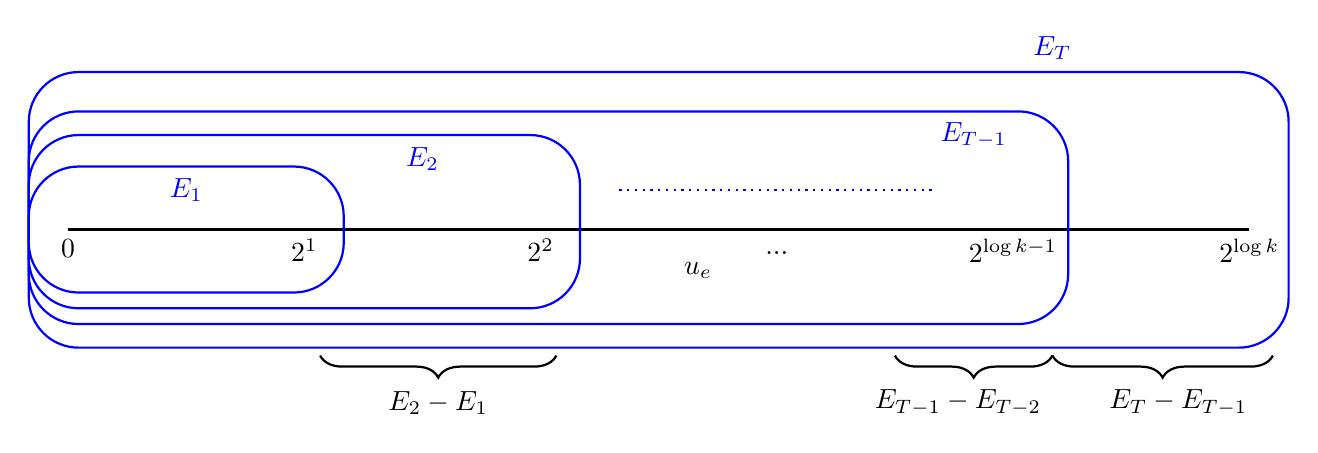
\begin{tikzpicture}

\def\PageWidth{15}
    
\draw[thick] (0,0) -- (\PageWidth,0);

\coordinate (A) at (0,0);
    \coordinate (B) at (3,0);
    \coordinate (C) at (6,0);
    \coordinate (D) at (12,0);
    \coordinate (E) at (\PageWidth,0);
    \coordinate (F) at (13.5,0); 

\draw[blue, thick, rounded corners=18pt] (-0.5,-0.8) rectangle (3.5,0.8);  \draw[blue, thick, rounded corners=18pt] (-0.5,-1) rectangle (6.5,1.2);  \draw[blue, thick, rounded corners=18pt] (-0.5,-1.5) rectangle (\PageWidth+0.5,2); \draw[blue, thick, rounded corners=18pt] (-0.5,-1.2) rectangle (12.7,1.5); 

\node at (A) [below] {$0$};
    \node at (B) [below] {$2^1$};
    \node at (C) [below] {$2^2$};
    \node at (D) [below] {$2^{\log k - 1}$};
    \node at (E) [below] {$2^{\log k}$};
    \node at (9,-0.3) {...};
    \node at (8,-0.3) [below] {$u_e$};

\node at (1.5,0.5) {\textcolor{blue}{$E_1$}};
    \node at (4.5,0.9) {\textcolor{blue}{$E_2$}};
    \node at (12.5,2.3) {\textcolor{blue}{$E_T$}};
    \node at (11.5,1.2) {\textcolor{blue}{$E_{T-1}$}};

\draw[thick,decorate,decoration={brace,amplitude=8pt,mirror}] (3.2,-1.6) -- (6.2,-1.6) node[midway,yshift=-0.6cm] {$E_2 - E_1$};
    \draw[thick,decorate,decoration={brace,amplitude=8pt,mirror}] (10.5,-1.6) -- (12.5,-1.6) node[midway,yshift=-0.6cm,xshift=-0.2cm] {$E_{T-1} - E_{T-2}$};
    \draw[thick,decorate,decoration={brace,amplitude=8pt,mirror}] (12.5,-1.6) -- (\PageWidth+0.3,-1.6) node[midway,yshift=-0.6cm,xshift=0.2cm] {$E_T - E_{T-1}$};

\draw[thick,blue,dotted] (7,0.5) -- (11,0.5);

\end{tikzpicture}
}
\end{figure}


Our algorithm will have $T$ iterations and each iteration (except
for the first and the last) will have two phases. During iteration~$i$,
we will be rounding some of the edges in the $i$-th bucket,
i.e., some of the edges in the set $E_{T-i+1} - E_{T-i}$.
Note that an edge $e$ in the $i$-th bucket has capacity $2^{T-i}<u_e\leq2^{T-i+1}$.

For every non-trivial cut $S$, we will maintain the following invariants for all iterations $i \in [2..(T-1)]$ (i.e. except the first and the last iteration):

\begin{enumerate}
    \item At the beginning of iteration $i$, $E_{cur} \cap E_{T-i+1} = \emptyset$ and
	$$\sum_{e\in E_{cur} \cap \delta(S)}u_e + \sum_{e\in E_{T-i + 1} \cap \delta(S)} \alphatwo\ u_ex^*_e \geq k.$$
We note that iteration $1$ ensures that this invariant holds at the start of iteration $2$.

    \item At the end of the first phase of iteration $i$,
    \[
    \sum_{e\in E_{cur} \cap \delta(S)}u_e + \sum_{e\in E_{T-i} \cap \delta(S)}\alphatwo\  u_ex^*_e \geq k-2^{T-i+1} - 2^{T-i}.
    \]

    \item At the end of iteration $i$, which is also the end of phase
    2 of iteration $i$, $E_{cur} \cap E_{T-i} = \emptyset$, and
    $$\sum_{e\in E_{cur} \cap \delta(S)}u_e + \sum_{e\in E_{T-i} \cap \delta(S)} \alphatwo\  u_ex^*_e \geq k.$$
\end{enumerate}

Observe that invariant~3 for iteration~$i$ is the same as invariant~1 for iteration~$i+1$.

Next, we present pseudo-code for the rounding algorithm, followed by explanation and analysis of the main steps.

{
\begin{algorithm}[H]
    \caption{$O(\log(k))$-approximate solution to Cap-$k$-ECSS}\label{alg:capkECSS}
    \begin{algorithmic}[1]
        \Require Graph $G = (V,E)$ with edge capacities $\{u_e\}_{e \in E}$ and costs $\{c_e\}_{e\in E}$.  A solution $x^*$ to \eqref{intro-KCLP:CapkECSS}, set $E_{cur} = \{e\in E:x^*_e \geq 1/2\}$, and sets $E_j \subseteq E, j = 1,...,\lceil \log k \rceil$ as defined above.

        \State Iteration 1:
        \begin{enumerate}[(a)]
        \item Let $\C = \{\emptyset\neq S \subsetneq V \; : \; \sum_{e \in E_{cur} \cap \delta(S)}u_e + \sum_{e \in E_{T-1} \cap \delta(S)} 2 u_e x^*_e < k\}$.  
        
        \item  Apply the approximation algorithm for $\ASC$ to select edges from $E - E_{T-1} - E_{cur}$ to cover the cuts in $\C$.  Add the selected edges to $E_{cur}$.

        \item Repeat (a), (b) once.
    \end{enumerate}

    \State For $i = 2,...,T-1$, Iteration $i$:
    \begin{enumerate}[(a)]
        \item For $\ell = 1,...,\lfloor (k-2^{T-i+1})/2^{T-i} \rfloor$:
        \begin{enumerate}[(i)]
            \item Let $\C = \{\emptyset\neq S \subsetneq V \; : \; \sum_{e \in E_{cur} \cap \delta(S)}u_e + \sum_{e \in E_{T-i} \cap \delta(S)} 2 u_e x^*_e < \ell\; 2^{T-i}\}$.  

            \item Apply the approximation algorithm for $\ASC$ to select edges from $E _{T-i+1}- E_{T-i} - E_{cur}$ to cover the cuts in $\C$.  Add the selected edges to $E_{cur}$.
        \end{enumerate}

        \item Let $\C = \{\emptyset\neq S \subsetneq V \; : \; \sum_{e \in E_{cur} \cap \delta(S)}u_e + \sum_{e \in E_{T-i} \cap \delta(S)} 2 u_e x^*_e < k\}$.  
            
        \item Apply the approximation algorithm for $\ASC$ to selected edges from $E - E_{T-i} - E_{cur}$ to cover the cuts in $\C$.  Add the selected edges to $E_{cur}$.

        \item Repeat (b), (c) \textbf{two} additional times.
    \end{enumerate}

    \State Iteration $T$:
    \begin{enumerate}[(a)]
        \item At this point, we have that $\sum_{e \in E_{cur} \cap \delta(S)}u_e + \sum_{e \in E_1 \cap \delta(S)}2 u_e x^*_e \geq k$ for all $S \subsetneq V, S \neq \emptyset$.  Apply Jain's iterative rounding method to round the edges in $E_1$ to an integer solution $E_1^*$, such that $E_{cur} \cup E_1^*$ is a feasible solution to Cap-$k$-ECSS.
    \end{enumerate}

    \State Return $E_{cur} \cup E_1^*$.
    \end{algorithmic}
\end{algorithm}
}



\paragraph{Iteration 1}

In this iteration, we consider the family of small cuts $S \subsetneq V$ where
\[
\sum_{e\in E_{cur} \cap \delta(S)}u_e+ \sum_{e\in E_{T-1} \cap \delta(S)}\alphatwo\  u_ex^*_e < k \tag{definition of small cuts}
\]

We will cover these cuts using edges in $E-E_{T-1} - E_{cur}$. Note
that the definition of small cuts above implies that $\sum_{e\in
E_{T-1} \cap \delta(S)}u_ex^*_e < R/\alphatwo$ where $R = k - \sum_{e\in E_{cur} \cap \delta(S)}u_e$.
The knapsack-cover inequality then implies that $\sum_{e\in (E-E_{T-1} - E_{cur}) \cap \delta(S)}
R x^*_e > R/\alphatwo$. Thus $\alphatwo\,x^*_{E-E_{T-1}
- E_{cur}}$ is feasible for the Cover Small Cuts problem implying
that we incur a cost of at most $5 \cdot \alphatwo \cdot c(x^*_{E_T-E_{T-1}})$
here. We add these edges to $E_{cur}$ and we repeat one more time,
i.e. we again consider all cuts where $\sum_{e\in E_{cur} \cap \delta(S)}u_e+
\sum_{e\in E_{T-1} \cap \delta(S)}\alphatwo u_ex^*_e < k$ and augment these cuts using
edges in $E-E_{T-1} - E_{cur}$, incurring a further cost of
$5 \cdot \alphatwo \cdot c(x^*_{E-E_{T-1}})$. Now, we will have necessarily satisfied
invariant 3 at the end of this iteration. Since, if this invariant were not satisfied for some cut, then this cut 
participated as a small cut in both instances of the $\ASC$ considered in this step.
This means we would have added at least two edges across this cut, each of capacity at least $k/2$, ensuring that invariant 3 holds.


\paragraph{Iteration $i$ Phase 1:} (Step 2 (a) in Algorithm \ref{alg:capkECSS})

We are starting with invariant 1 at the beginning of this iteration
(as this corresponds to the invariant 3 that holds at the end of the previous iteration). Hence we
have $E_{cur} \cap E_{T-i+1} = \emptyset$ and $\sum_{e\in E_{cur}}u_e
+ \sum_{e\in E_{T-i + 1}} \alphatwo u_ex^*_e \geq k$. We will run
multiple sub-iterations within this phase. Let's describe the first
sub-iteration.

Consider the family of small cuts $S \subsetneq V$ where $\sum_{e\in E_{cur} \cap \delta(S)}u_e +
\sum_{e\in E_{T-i} \cap \delta(S)} \alphatwo u_ex^*_e < 2^{T-i}$. We will cover these
cuts using edges in $E_{T-i+1}-E_{T-i}-E_{cur}$. For these small cuts, we must have 
$$\sum_{e\in (E_{T-i+1}-E_{T-i}-E_{cur}) \cap \delta(S)}\alphatwo
u_ex^*_e \geq k-2^{T-i},$$ 
since invariant 1 is true. Note that
$u_e \leq 2^{T-i+1}$ for all edges in $E_{T-i+1}$ and so $\sum_{e\in
(E_{T-i+1}-E_{T-i}-E_{cur}) \cap \delta(S)}\alphatwo x^*_e \geq (k-2^{T-i})/2^{T-i+1}$.
Thus, $\alphatwo x^*_{E_{T-i+1}-E_{T-i}-E_{cur}} \cdot 2^{T-i+1}/(k-2^{T-i})$
is feasible for the Cover Small Cuts problem. We add the (approximate)
solution of the Cover Small Cut problem to $E_{cur}$. Note that
after this, there are no cuts $S \subsetneq V$ with $\sum_{e\in E_{cur} \cap \delta(S)}u_e +
\sum_{e\in E_{T-i} \cap \delta(S)} \alphatwo u_ex^*_e < 2^{T-i}$ since we would have
added an edge from $E_{T-i+1}-E_{T-i}-E_{cur}$ to $E_{cur}$ and all
these edges have capacity at least $2^{T-i}$. We now shift the
threshold in the definition for Small Cuts to $2\cdot 2^{T-i}$, and
then to $3\cdot 2^{T-i}$, all the way until $\hat{\ell}\cdot 2^{T-i}$
where $\hat{\ell} = \lfloor (k-2^{T-i+1})/2^{T-i} \rfloor$. This
would imply that  $\hat{\ell}\cdot2^{T-i}\geq k-2^{T-i+1} - 2^{T-i}$.
We describe these sub-iterations in more detail now.

For $\ell = 1,2,\ldots, \hat{\ell}$, consider the family of small cuts $S \subsetneq V$ where
\[
\sum_{e\in E_{cur} \cap \delta(S)}u_e + \sum_{e\in E_{T-i} \cap \delta(S)} \alphatwo u_ex^*_e < \ell\cdot 2^{T-i} \tag{definition of small cuts}
\]
Since invariant 1 is true (and we have only increased the LHS of
invariant 1 during the phase), it must be true that
\[
\sum_{e\in (E_{T-i+1}-E_{T-i}-E_{cur}) \cap \delta(S)}\alphatwo  u_ex^*_e \geq k-\ell\cdot 2^{T-i}
\]
Since $u_e \leq 2^{T-i+1}$ for all edges in $E_{T-i+1}$, we must have
\[
\sum_{e\in (E_{T-i+1}-E_{T-i}-E_{cur}) \cap \delta(S)}\alphatwo  x^*_e \geq (k-\ell\cdot 2^{T-i})/2^{T-i+1}
\]
Thus, $\alphatwo x^*_{E_{T-i+1}-E_{T-i}-E_{cur}} \cdot 2^{T-i+1}/(k-\ell\cdot
2^{T-i})$ is feasible for our instance of the Cover Small Cuts problem. We add
an (approximate) solution of this Cover Small Cuts problem to
$E_{cur}$, and move on to the next sub-iteration. At the end of all
the sub-iterations, it must be true that
\[
    \sum_{e\in E_{cur} \cap \delta(S)}u_e + \sum_{e\in E_{T-i} \cap \delta(S)}\alphatwo u_ex^*_e \geq (\hat{\ell})2^{T-i} \geq k-2^{T-i+1}-2^{T-i}
\]
and so invariant 2 is maintained. Let us analyze the cost we incurred in this phase.

The cost we incur is at most $5 \cdot \alphatwo \cdot  c(x^*_{E_{T-i+1}-E_{T-i}})2^{T-i+1}
(\frac{1}{k-2^{T-i}} + \frac{1}{k-2\cdot2^{T-i}} +
\cdots+\frac{1}{k-\hat{\ell}2^{T-i}})$. We bound this last sum as
follows. Note that $\hat{\ell} 2^{T-i} \leq k - 2^{T-i+1}$ and so
$k-\hat{\ell}2^{T-i} \geq 2^{T-i+1}$.
\begin{align*}
    &\frac{1}{k-2^{T-i}} + \frac{1}{k-2\cdot2^{T-i}} + \cdots+\frac{1}{k-\hat{\ell}2^{T-i}} \\
    &= \frac{1}{k-\hat{\ell}2^{T-i}} + \frac{1}{k-\hat{\ell}2^{T-i} + 2^{T-i}}+ \frac{1}{k-\hat{\ell}2^{T-i} + 2\cdot 2^{T-i}} + \cdots \frac{1}{k-\hat{\ell}2^{T-i} + (\hat{\ell}-1)\cdot 2^{T-i}}\\
    &\leq \frac{1}{2^{T-i+1}} + \sum_{\theta = 1}^{\hat{\ell}-1} \frac{1}{k-\hat{\ell}2^{T-i} + 2^{T-i}\theta}\\
    &\leq \frac{1}{2^{T-i+1}} + \int_0^{\hat{\ell}-1} \frac{1}{k-\hat{\ell}2^{T-i} + 2^{T-i}\theta} d(\theta)\\
    & = \frac{1}{2^{T-i+1}}+ \frac{1}{2^{T-i}}\left(\log(k-2^{T-i}) - \log(k-\hat{\ell}2^{T-i})\right)\\
    & = O(\frac{\log k}{2^{T-i}})
\end{align*}
Thus, the total cost we incur in this phase is at most
$(5)(\alphatwo) (2^{T-i+1}/2^{T-i})O(\log k) c(x^*_{E_{T-i+1}-E_{T-i}})$.

\paragraph{Iteration $i$ Phase 2:} (Step 2 (b)-(d) in Algorithm \ref{alg:capkECSS})

We are beginning with invariant 2, which is valid at the end of phase 1, and thus for all cuts $S \subsetneq V$, we have

\[
    \sum_{e\in E_{cur} \cap \delta(S)}u_e + \sum_{e\in E_{T-i} \cap \delta(S)}\alphatwo u_ex^*_e \geq k-2^{T-i+1} - 2^{T-i}
\]
We will add more edges from $E-E_{T-i}-E_{cur}$ to these cuts, if needed, to
increase the connectivity to $k$. Note that all edges in
$E-E_{T-i}-E_{cur}$ have capacity at least $2^{T-i}$ and so at most three more edges need to be added. To do so, we employ the same
technique as iteration 1.

Consider the family of small cuts $S \subsetneq V$ where
\[
\sum_{e\in E_{cur} \cap \delta(S)} u_e + \sum_{e\in E_{T-i} \cap \delta(S)}\alphatwo u_e x^*_e <k
\]
Then, by the knapsack-cover inequalities,
$\alphatwo\,x^*_{E-E_{T-i}-E_{cur}}$ is feasible for
the $\ASC$ instance. Indeed for these small cuts, we have $\sum_{e\in
E_{T-i} \cap \delta(S)}u_ex^*_e < R/\alphatwo$ where $R = k - \sum_{e\in E_{cur}}u_e$.
The knapsack-cover inequality then implies that $\sum_{e\in (E-E_{T-i} - E_{cur}) \cap \delta(S)}
R x^*_e > R/\alphatwo$. Hence, we can solve this Cover Small Cuts instance incurring a cost of at most $10c(x^*_{E-E_{T-i}-E_{cur}})$.

We do so thrice, adding the approximate solution
of the $\ASC$ instance to $E_{cur}$ and incur a cost of at most
$3\times 10c(x^*)$. At the end of this phase, it must be true that for any cut $S \subsetneq V$, we have
\[
\sum_{e\in E_{cur} \cap \delta(S)}u_e + \sum_{e\in E_{T-i} \cap \delta(S)}\alphatwo u_e x^*_e \geq k.
\]
This is precisely invariant 3 and we have completed this phase.

\paragraph{Iteration $T$}

In the beginning of the last iteration, we have for any cut $\emptyset \subsetneq S \subsetneq V$:
\[
\sum_{e\in E_{cur} \cap \delta(S)}u_e + \sum_{e\in E_{1} \cap \delta(S)}\alphatwo u_e x^*_e \geq k.
\]
But now, we can employ Jain's iterative rounding framework to round
the edges in $E_1$, incurring a cost of at most
$(2\max\{u_e: e\in E_1\})c(x^*_{E_1}) = 4c(x^*_{E_1})$.


\paragraph{Solving the LP Relaxation:} 
Given a feasible optimal solution $x^*$ to \eqref{intro-KCLP:CapkECSS}, our rounding algorithm is easily seen to run in polynomial-time. However, it remains to show that we can compute the desired solution  $x^*$ in polynomial-time.
As before, we would like solve the above LP using the ellipsoid method, but we unfortunately do not know a polynomial-time separation oracle for the entire set of knapsack-cover inequalities. We will instead {\em iteratively} identify a subset of edges $A$, and a polynomial-time computable collection of cuts such that as long as knapsack-cover inequalities hold for this collection, we will be able to execute the rounding algorithm. In what follows, we assume w.l.o.g.\ that the optimal LP solution cost, say $\lpopt$, is known as it can be identified by running binary search. We can thus replace the minimization objective with simply a feasibility constraint on our solution, namely $\sum_{e\in E}c_e x_e \leq \lpopt$.


\begin{lemma}\label{lem:polytimeKC_CapkECSS}
There is a polynomial-time algorithm that computes a solution $x^*$ to \eqref{intro-KCLP:CapkECSS} of value at most $\lpopt$ such that for every iteration $i \in [1..(T-1)]$, the solution $x^*$ satisfies the property that $2x^*_{E-E_{T-i} - E_{cur}}$ is feasible for the Cover Small Cuts instances created in steps 1(b), and 2(c) of Algorithm~\ref{alg:capkECSS}. 
\end{lemma}
\begin{proof}\textcolor{red}{TOPROVE 6}\end{proof}


\begin{theorem} \label{thm:approx-CapkECSS}
Let $\opt$ be the optimal solution value for a given instance of Cap-$k$-ECSS. Then there is a polynomial-time algorithm that computes a solution $x^*$ to \eqref{intro-KCLP:CapkECSS} of value at most $\opt$ (possibly satisfying only a subset of the constraints) and rounds it to obtain a feasible integer solution of cost at most $O(\log k) \cdot \opt$
\end{theorem}

}

\clearpage

\begin{appendices}
\section{Formulating $\pqfgc$ as a Cap-$k$-ECSS Problem \label{sec:A1:pqfgc}}
{
We attempt to model $\pqfgc$ as the Cap-$k$-ECSS problem.
Let us take $p$ and $q$ to be parameters.
Our goal is to find conditions on $p$ and $q$ such that $\pqfgc$
can be formulated as a Cap-$k$-ECSS problem.
We show that one can formulate a $\pqfgc$ problem as an equivalent
Cap-$k$-ECSS problem if and only if $p=1$ or $q=1$.

We make the following assumptions:

\begin{itemize}
\item
$p$ and $q$ are positive integers;
\item
each unsafe edge is assigned the capacity $u(p,q)>0$;
\item
each safe edge is assigned the capacity $s(p,q)\geq u(p,q)>0$;
\item
the requirement $k$ of the Cap-$k$-ECSS problem is fixed at
$p \cdot s(p,q) = (p+q) \cdot u(p,q)$, because each nontrivial cut
of $\pqfgc$ is required to have either $p$ safe edges or $p+q$ edges.
\end{itemize}

Clearly, a cut that violates the requirement of $\pqfgc$ should
have capacity less than $k$.
Let us call this property~(0).

For any $i = 1,2,...,p-1$, a cut does not satisfy the requirement
of $\pqfgc$ if it has $\leq p-i$ safe edges and $\leq q+i-1$ unsafe edges.

This gives the constraint $(p-i)s(p,q) + (q+i-1)u(p,q) < k$.

Since $k = p\cdot s(p,q) = (p+q)\cdot u(p,q)$, we have  $s(p,q) =
u(p,q)(p+q)/p$. Starting from property~(0), we get the following
(each line follows from the preceding line):

\begin{align*}
(p-i) s(p,q) + (q+i-1) u(p,q) &\quad <\quad k = (p) s(p,q) \\
(-i) s(p,q) + (q+i-1) u(p,q) &\quad <\quad 0 \\
(-i)  u(p,q) \frac{p+q}{p} + (q+i-1) u(p,q) &\quad <\quad 0 \\
\text{Since $u(p,q)>0$, this is equivalent to} & \\
q+i-1 &\quad <\quad (i)  \frac{p+q}{p} \\
pq+ip-p &\quad <\quad (i) (p+q) \\
pq &\quad <\quad iq + p \qquad (\text{inequality}~(*)) \\
\end{align*}


Recall that $i \in \{1,...,p-1\}$.
Suppose that $i=1$ and assume that $q\geq p$.
Then inequality~($*$) is the same as
$\displaystyle p < 1 + \frac{p}{q} \leq 2$, that is, $p \leq 1$.
Thus, inequality~($*$) implies either $q < p$ or $p = 1$.

Similarly, by taking $i=1$ and assuming that $p\geq q$, inequality~($*$) can be written as
$\displaystyle q < 1 + \frac{q}{p} \leq 2$, that is, $q \leq 1$.
Thus, inequality~($*$) implies either $p < q$ or $q = 1$.

Hence, either $p=1$ or $q=1$ (since $p < q$ and $q < p$ cannot both be true).
}
\section{An $O(p\log{n})$-Approximation Algorithm for $\pqfgc$ via Covering Integer Programs \label{sec:A2:log-approx}}
{
We apply a theorem from Chekuri \& Quanrud \cite{CQ:soda19} that gives
an approximation algorithm for Covering Integer Programs (abbreviated as CIPs).
We recap Theorem~2.3 from \cite{CQ:soda19}.

\medskip

\noindent
\textbf{Theorem} [Chekuri \& Quanrud \cite{CQ:soda19}]
\textit{Given $A\in[0,1]^{m\times{n}}$, $c\in\Rp^n$, $d\in\Zp^n$, $x\in\Rp^n$,
such that $x$ satisfies the Knapsack Cover Inequalities.
Let the approximation parameter be $\alpha = \ln\Delta_0+\ln\ln\Delta_0+O(1)$.
The algorithm runs in time $\|A\|_0$ and finds an integer vector $z$
of cost $\leq \alpha \cdot c^\top x$ such that $Az\geq 1$ and $0\leq z\leq d$.
(Here, $\|A\|_0$ denotes the number of nonzeros of $A$, and $\Delta_0$
denotes the maximum number of nonzeros in any column of $A$.)
}
\\
(Note: for our application to $\pqfgc$, we take $\Delta_0 = |V(G)| = \hat{n}$.)

\bigskip

We apply the theorem from \cite{CQ:soda19} to cover the deficient cuts
while augmenting a solution to $(i,q)$-FGC to a solution to $(i+1,q)$-FGC.
We have two types of deficient cuts:

\begin{itemize}
\item[(1)]
Cuts with exactly $(i+q)$ edges (safe or unsafe);
we need to pick one more edge (safe or unsafe) to cover each such cut.

\item[(2)]
Cuts with exactly $i$ safe edges and $j$ unsafe edges, where $j\in\{0,1,2,\dots,q-1\}$;
for each such cut, we need to pick either one safe edge or $(q+1-j)$ unsafe edges;
we can formulate this requirement as a valid inequality constraint of a CIP
such that we can apply the theorem of \cite{CQ:soda19}.

\item[]
(Note: if a cut has $i$ safe edges and $q$ unsafe edges, then it is a cut of type~(1)).
\end{itemize}

The algorithm starts by computing a (1,q)-FGC solution of cost $O(\log{n})\opt$.
In detail, we formulate (precisely) the (1,q)-FGC problem as a
Capacitated Network Design (CND) problem,
by assigning capacities of $(q+1)$ and one, respectively, to the safe~edges and the unsafe~edges.
Then, we apply the $O(\log{n})$ approximation algorithm of Chakrabarty et~al.\ \cite{CCKK15}
to our CND~problem.

Next, we apply $p-1$ iterations. Iteration~$i$ starts with a solution to $(i,q)$-FGC
and augments deficient cuts (if any) to obtain a solution to $(i+1,q)$-FGC.
Each iteration formulates a CIP and finds a solution to this CIP
of cost $O(\log{n})\opt$, using the algorithm/theorem of \cite{CQ:soda19}.

Thus, the overall approximation ratio is $O(p\log{n})$.

We present the details for iteration~$i$ in what follows.
Let $H$ be the solution to $(i,q)$-FGC, at the start of the iteration.
Our goal is to find all the deficient cuts, then write down a CIP,
then find an approximately optimal solution to the CIP via \cite[Theorem~2.3]{CQ:soda19}.
We start by formulating a CND using the following parameters:

\medskip

\centerline{
\begin{tabular}{|lr|} \hline
capacity of a safe edge:\quad &		$i+q$ \\
capacity of an unsafe edge:\quad &	$i$ \\
required capacity (for each non-trivial cut):~~ & $i(i+q)$ \\ \hline
\end{tabular}
}
\medskip

Observe that the CND graph (corresponding to $H$) has capacity $\ge i(i+q)$ for
every non-trivial cut, because $H$ is a solution to $(i,q)$-FGC.

\begin{claim}
If a cut of the CND graph has capacity $\geq 2(i+1)(i+q)$,
then this cut satisfies the requirement of $(i+1,q)$-FGC.
\end{claim}
\begin{proof}\textcolor{red}{TOPROVE 7}\end{proof}

We apply the algorithm of Nagamochi, Nishimura, \& Ibaraki \cite{NNI97}
to list all the cuts in the CND graph
with capacities in the range $[i(i+q),\;2(i+1)(i+q)]$
in (deterministic) polynomial time.
Note that $2(i+1)(i+q) \leq 4 i(i+q)$, hence, by Karger's results,
the number of cuts in this range is $O(n^8)$.

Finally, we set up the constraints matrix $A$ for the CIP.
For each deficient cut $\delta(S_k)$ (in our list of cuts of the CND graph),
we write a constraint of the form $\row_k(A) \cdot x \geq b_k$.
For a deficient cut of type~(1), i.e., a cut with $i+q$ edges,
we have the constraint $\sum_{e\in\delta(S_k)\cap{(E(G)-E(H))}}x_e\geq1$.

Next, for notational convenience, define $a_j = (q+1-j)$.
For a deficient cut of type~(2), i.e., a cut with $i$ safe edges and $\leq q-1$ unsafe edges,
let $j\in\{0,\dots,q-1\}$ denote the number of unsafe edges;
for each unsafe edge $e\in E(G)-E(H)$ we fix the coefficient $A_{k,e} = 1$, and
for each safe edge $f\in E(G)-E(H)$ we fix the coefficient $A_{k,f} = a_j$,
and we fix the RHS coefficient $b_k = a_j$.
Thus, we have the constraint
\[	a_j \, \sum_{f\in\delta(S_k)\cap\safe\cap{(E(G)-E(H))}}x_f +
        \sum_{e\in\delta(S_k)\cap\unsafe\cap{(E(G)-E(H)})}x_e \geq{a_j}.
\]
}


\end{appendices}
\bibliographystyle{plainurl}
\bibliography{cnd-fgc-arxiv}

\end{document}
